\chapter{Literature Review} \label{chap:state_art}

\section*{}

In this chapter we discuss some key concepts related to e-commerce, for the 
purpose of giving context to the dissertation. We discuss the typical customer 
life cycle in an e-commerce website, some metrics that might be used and some 
ways on how the customer interaction with the website might be influenced and 
improved.

\section{E-commerce background} \label{chap:ecommerce}

\subsection{Introduction}

E-commerce, or electronic commerce, can be described by the trading of products 
or services over the Internet (or other computer networks). The type of 
e-commerce businesses we are interested are those who sell their goods directly 
to the customer, e.g online shopping, using an online store or catalog of 
products. Some popular online 
stores\footnote{\url{http://www.alexa.com/topsites/category/Top/Shopping}} are 
Amazon\footnote{\url{http://www.amazon.com/}}, 
Ebay\footnote{\url{http://www.ebay.com/}} and 
Alibaba\footnote{\url{http://www.alibaba.com/}}.

\subsection{Customer life cycle}

An important concept to understand the customer is by describing its life 
cycle, as presented by~\cite[Section 6]{Sterne2000} in 
figure~\ref{fig:lifecycle}.

\begin{figure}[h]
  \begin{center}
    \leavevmode
    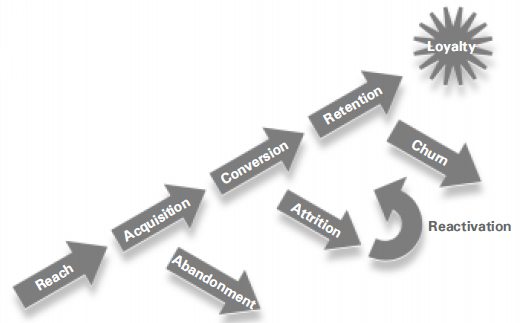
\includegraphics[width=0.86\textwidth]{lifecycle}
    \caption{Customer lifecycle \cite{Sterne2000}}
    \label{fig:lifecycle}
  \end{center}
\end{figure}

It starts by reaching the target audience or market up to an established 
customer base, not forgetting about those that drop mid way, due to abandonment 
or attrition.

\begin{itemize}
    \item Reach happens outside of the website and refers to the number of 
    potential customers. For example, if the online store is advertised on a 
    social network, the reach is the number of users who were served the ad in 
    that other website, they may or may not ignore it.
    \item Acquisition is the next stage, where the user decides to act on and 
    visits the website (or some other action like subscribing to a newsletter).
    \item Conversion is the stage where a visitor stops being a user and starts 
    being a customer. It usually means that the user made a purchase but some 
    companies might consider a sign up or registration in the website as a 
    conversion.
    \item Retention focuses on making existing customers, that made at least 
    one purchase before, repeat purchases.
    \item Loyalty is a stronger form of retention, which represents a greater 
    trust level of the customer in the store.
    \item Abandonment is defined by the customers that started the buying 
    process but do not finish it. For example, a customer may add items to the 
    online shopping cart but instead of moving to the next step, e.g. enter 
    credit card details, they exit the website or go elsewhere. This may happen 
    in any store with a multi-step buying process, which is very common.
    \item Attrition happens when a retained customer ceases buying from the 
    store and starts using a competitor store.
    \item Churn is defined by the number of customer that attrited during a 
    certain period divided by the total number of customers at the end of that 
    period. It measures how much of the customer base "rolls over" in a certain 
    time period.
\end{itemize}

\subsection{Customer Behaviour Model Graph (CBMG)}

A state transition graph named Customer Behaviour Model Graph (CBMG) can be 
used to describe the behaviour of customers browsing a website. The nodes 
represent the possible states or pages, e.g home page, product page, search, 
and a probability is associated with each transition. An example of such a CBMG 
is shown in figure \ref{fig:cbmg}.

\begin{figure}[h]
    \begin{center}
        \leavevmode
        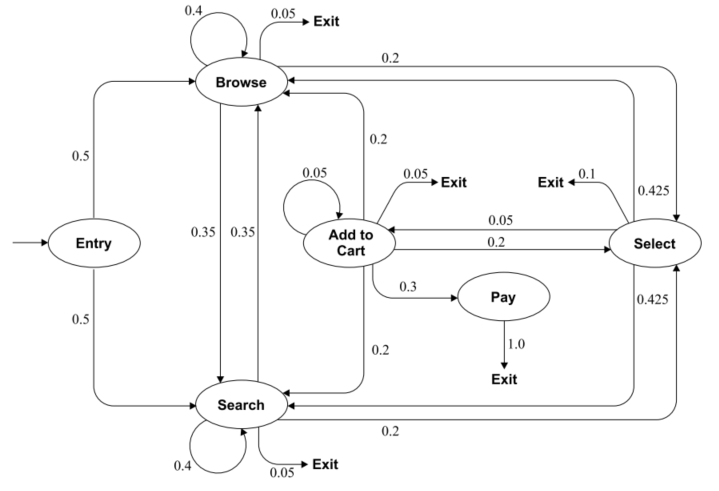
\includegraphics[width=0.86\textwidth]{cbmg}
        \caption{Example of a customer behaviour model graph \cite{Menasce1999}}
        \label{fig:cbmg}
    \end{center}
\end{figure}

\cite{Menasce1999} describes how CBMGs can be used to analyse the workload of 
an e-commerce store server and how metrics can be derived directly from the 
CBMG alone.

\subsection{E-commerce metrics}

Metrics are a common way to quantify, measure, benchmark or evaluate some 
process. In an e-commerce setting, businesses are interested in optimizing, 
mostly, for profit. Different businesses prioritize metrics in different ways, 
adapted to each use case. Here we present some common used metrics, but this 
list is by no means exhaustive. \cite{Sterne2000, Menasce1999}

\begin{itemize}
    \item \textit{Conversion Rate} (CR) is the percentage of visitors that buy 
    a product or a service;
    \item \textit{Shopping Cart Abandonment} is the percentage of visitors that 
    added a product to the online cart but did not complete the process;
    \item \textit{Average Order Value} (AOV) is the average size of an order;
    \item \textit{Customer Lifetime Value} (LTV) is the projected value that a 
    customer will spend on the store;
    \item \textit{Clicks to Buy} (CTB) is the average number of clicks a 
    visitor has to do to complete a buy order;
    \item \textit{Churn Rate} the percentage of customers that do not make a 
    repeated purchase;
    \item \textit{Bounce Rate} is the percentage of visitors that arrive at the 
    homepage of the online store but leave immediately, without clicking 
    anything or visiting a different page.
\end{itemize}

There are other common metrics such as \textit{Acquisition Cost}, \textit{Cost 
Per Conversion}, \textit{Net Yield} or \textit{Connection Rate} however they 
are associated with promotion campaigns that happen outside of the store 
website, therefore they are not interesting in the context of our work.

\subsection{Influencing user behaviour}

Tracking a bunch of statistics and metrics about an online store is no good if 
there are no actionable changes that can be done using that information. 
\cite{Constantinides2004} describes functionality, psychological and content 
factors that can influence the visitor experience, represented in the table 
\ref{tab:factors}.

\begin{table}[h]
    \centering
    \caption{Main building blocks of Web experience and their sub-categories 
    \cite{Constantinides2004}}
\label{tab:factors}
\begin{tabular}{lll}
    \cline{1-2}
    \multicolumn{2}{|c|}{\textbf{Functionality 
    factors}}                                               & 
    \textbf{}                                   \\ \cline{1-2}
    \multicolumn{1}{|l|}{\textbf{Usability}}             & 
    \multicolumn{1}{l|}{\textbf{Interactivity}} & 
    \textbf{}                                   \\ \cline{1-2}
    Convenience                                          & Customer 
    service/after sales                
    &                                             \\
    Site navigation                                      & Interaction with 
    company personnel          &                                             \\
    Information architecture                             & 
    Customization                               &                               
                  \\
    Ordering/payment process                             & Network 
    effects                             &                                       
          \\
    Search facilities and process                        
    &                                             &                             
                    \\
    Site speed                                           
    &                                             &                             
                    \\
    Findability/accessibility                            
    &                                             &                             
                    \\
    &                                             
    &                                             \\ \hline
    \multicolumn{1}{|c|}{\textbf{Psychological factors}} & 
    \multicolumn{2}{c|}{\textbf{Content 
    factors}}                                             \\ \hline
    \multicolumn{1}{|l|}{\textbf{Trust}}                 & 
    \multicolumn{1}{l|}{\textbf{Aesthetics}}    & 
    \multicolumn{1}{l|}{\textbf{Marketing mix}} \\ \hline
    Transaction security                                 & 
    Design                                      & 
    Communication                               \\
    Customer data misuse                                 & Presentation 
    quality                        & 
    Product                                     \\
    Customer data safety                                 & Design 
    elements                             & 
    Fulfillment                                 \\
    Uncertainty reducing elements                        & 
    Style/atmosphere                            & 
    Price                                       \\
    Guarantees/return policies                           
    &                                             & 
    Promotion                                   \\
    &                                             & 
    Characteristics                            
\end{tabular}
\end{table}

Regarding usability of the online store, providing a personalized experience to 
each customer can be very beneficial for both the customer and the business. A 
common way to do this is by recommending products that the customer might be 
interested it \cite{Adomavicius2005}. For example, if we know that a customer 
buys mostly football related products, recommending her more products in the 
same category might increase sales.

\subsection{Summary}

In this chapter we covered a brief overview of e-commerce, starting with the 
customer lifecycle, how to measure it using metrics and presenting a common way 
to model the users' behaviour, the CBMG.

\section{System Simulation} \label{sec:simulation}

This chapter intends to introduce some approaches to computational simulation 
systems and engines, namely agent based and discrete event simulation. To 
finish the chapter, we show some novel approaches to simulation.

\subsection{Introduction}

Simulations are used to reproduce the behaviour of a system. They have been 
applied to different areas like physics, weather, biology, economics and many 
others. There are many types of simulations: stochastic or deterministic, 
steady-state or dynamic, continuous or discrete and local or distributed 
\cite{WKSimulation}. These categories are not exhaustive nor exclusive.

In this literature review, we are particularly interested in studying 
simulations which can model stochastic processes and not dynamic (dynamic 
systems are usually described by differential equations and are continuous).

\subsection{Agent Based Simulation (ABS)}

In agent based simulation (ABS), sometimes described as agent based computing 
\cite{wooldridge1998agent, jennings1999agent}, the individual entities in the 
model are represented discretely and maintain a set of behaviours, beliefs or 
rules that determine how their state is updated. \cite{Niazi2011} lists three 
different approaches to agent based modelling and simulation:

\begin{itemize}
    \item \emph{Agent-oriented programming} which puts emphasis on developing 
    complex individual agents rather than a large set of agents;
    \item \emph{Multi-agent oriented programming} focus on adding \emph{some} 
    intelligence to agents and observe their interactions;
    \item \emph{Agent-based or massively multi-agent modelling} where the main 
    idea is to build simple models for the agents which interact with a large 
    population of other agents to observe the global behaviour.
\end{itemize}

\cite{Siebers2010} describes ABS as ``well suited to modelling systems with 
heterogeneous, autonomous and pro-active actors, such as human-centred 
systems.'', which make them a good candidate to be used in the development of 
this dissertation. However, existing literature is quite confusing and broad, 
using different terms to refer to the same concepts, without clear 
distinctions between different agent based approaches and without consensus 
\cite{Niazi2011, Brailsford2014}.

Many platforms and frameworks were developed to support agent-based modelling 
and similation. Some notable examples include Repast~\cite{collier2003repast}, 
NetLogo~\cite{wilensky1999netlogo}, StarLogo~\cite{resnick1996starlogo} or 
MASON~\cite{panait2005cooperative}. An updated list is maintained at OpenABM 
\cite{OpenABM2016}.

Agents have been applied to e-commerce context mostly in two distinct areas: 
recommendation systems \cite{xiao2007commerce, walter2008model} and negotiation 
\cite{rahwan2002intelligent, maes1999agents}. No relevant literature was found 
regarding simulating user behaviour in websites with agents.

\subsection{Multi-agent interaction}

...

\subsection{Discrete Event Simulation (DES)} \label{ssec:des}

A discrete event simulation (DES) models a process as a series of discrete 
events, where the state of the system changes only at well defined points in 
time \cite{Siebers2010}. It was originally proposed by Kiviat in 1969 
\cite{Kiviat1969} and there is extensive research in this simulation technique. 
Banks et al. \cite{Banks2004} provides a comprehensive description and analysis 
of DES. The algorithm \ref{alg:des} is a possible implementation of a very 
simple and single-threaded DES.

\begin{algorithm}[h]
    \caption{Basic DES algorithm}
    \label{alg:des}
    %later in the document
    \begin{algorithmic}
        \State $EndCondition \gets false$
        \State $Clock \gets 0$
        \State $EventList \gets initialEvent$
        \While{$EndCondition = false$}
        \State $CurrentEvent \gets \Call{Pop}{EventList}$
        \State $Clock \gets \Call{Time}{CurrentEvent}$
        \State $\Call{Execute}{CurrentEvent}$ \Comment{might put new 
            events in $EventList$}
        \State $\Call{UpdateStatistics}$
        \EndWhile
        \State $\Call{GenerateReport}$
    \end{algorithmic}
\end{algorithm}

The major concepts in DES are as follows \cite{Banks2004}:

\begin{itemize}
    \item Entity, objects explicitly represented in the model (e.g, a customer);
    \item Event, an occurrence that changes the state of the system (e.g, a  
    customer enters the website);
    \item Event list (or future event list or pending event set), a list of 
    future events, ordered by time of occurrence;
    \item Clock, used to keep track of the current simulation time.
\end{itemize}

Event list is one of the fundamental parts of the system and it has been widely 
researched \cite{Henriksen1986, Jones1986, Tan2000, Dickman2013}.

Pidd \cite{pidd1998computer} proposes a three-phased approach that consists of: 
jump to the next chronological event, executing all the unconditional events 
(or type B) that happen that moment and then executing all the conditional 
events (or type C). This approach has advantages in terms of less usage of 
resources compared to other simplistic approaches. Also, there has 
been studies on how to scale DES to distributed and parallel (PDES)
executions~\cite{Misra1986, Fujimoto1990}.

\cite{SiebersDES2010} states that ``DES is useful for problems (...) in which 
the processes can be well defined and their emphasis is on representing 
uncertainty through stochastic distributions'', which makes DES a good 
candidate to model the problem at hand.

\subsection{Hybrid and novel approaches}

In recent years, there has been research which proposes a marriage between 
agent based model and simulation with discrete event simulation, however, this 
concept is not widely recognized \cite{Brailsford2014}. Brailsford states that 
the line that divides agent based models (and simulation) and DES is spurious 
and that common distinctions between the two approaches are artificial. Casas 
et al. \cite{FonsecaiCasas2011} describe a method where multi agent system 
components have been added to an existing discrete event simulation implemented 
in OMNeT++\footnote{C++ based discrete event simulation 
    toolkit}\cite{Varga2001}. Onggo \cite{Onggo2007} shows how agent based 
    models 
can be ran on top of a DES engine. Kurve et al.~\cite{Kurve2013} describes an 
agent based performance model of a PDES kernel. Regarding existing software, 
AnyLogic claims to be ``the only simulation tool that supports Discrete Event, 
Agent Based, and System Dynamics Simulation''~\cite{AnyLogic2000}. AnyLogic was 
first shown in 2000 at the Winter Simulation Conference.

\subsection{Summary}

This literature reviews shows that there is vast research regarding simulation, 
either agent based or DES, however not everyone is speaking the same language. 
The extensions to DES seen above are particularly interesting since they can be 
used to scale the simulation to a greater number of entities as well as 
modelling real world processes with more fidelity.

\section{Probabilistic Models} \label{sec:models}

\subsection{Introduction}

Probabilistic or statistical models represent explicit assumptions about a 
problem domain, in the form of a model. This model usually encompasses random 
variables\footnote{Variable whose value is given by a probability distribution, 
commonly represented by $\Theta$.}, in the form of probability distributions,  
and the relation and dependence between the variables.~\cite{Winn2013}

In the following sections we describe a common way to represent probabilistic 
models, probabilistic graphical models (PGM) or, simply, graphical models.

\subsection{Probabilistic Graphical Models}

A PGM is a graph based model where the nodes represent random variables and the 
(directed or undirected) edges represent a conditional dependence between 
variables. An example is shown in figure~\ref{fig:pgm}.

\begin{figure}[h]
    \begin{center}
        \leavevmode
        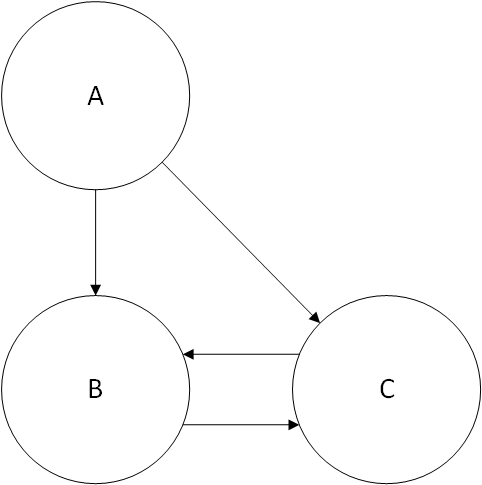
\includegraphics[width=0.36\textwidth]{pgm}
        \caption{Example of a PGM: B and C depend on A, B depends on C and C 
            depends on B.}
        \label{fig:pgm}
    \end{center}
\end{figure}

PGMs and their extensions, where we show some examples of them in the following 
sections, are exceptionally well suited for reasoning and to reach conclusions 
based on available information (both domain expert and data), even in the 
presence of uncertainty. PGMs provide a general framework that allows 
representation, inference and learning on these 
models.~\cite{koller2009probabilistic}

There is extensive research and available literature in this area. Some notable 
examples include, but are not limited to, the books \textit{"Probabilistic 
    Graphical Models: Principles and Techniques"} by Daphne Koller and Nir 
Friedman~\cite{koller2009probabilistic} and \textit{"Pattern Recognition and 
    Machine Learning"} (Chapter 8: Graphical Models) by Christopher 
Bishop~\cite{bishop2006pattern}. It is also worth mentioning that there is a 
MOOC \footnote{Massive Open Online Course} named \textit{"Probabilistic 
    Graphical Models"}, also by Daphne Koller (Stanford), freely available on 
Coursera \footnote{\url{https://www.coursera.org/course/pgm}}.

In the following sections, we describe three important categories of graphical 
models: Bayesian networks, Markov random fields and its extension to hidden 
Markov models. There are plenty of other graphical models however they were 
deemed not relevant enough to be included in this literature review.

\subsection{Bayesian Networks}

Bayesian networks, also named directed graphical models, is a type of PGM where 
the edges in the graph representation are directed and represent causal 
relationships between random variables or group of random variables (see figure 
\ref{fig:pgm}). This concept was first introduced by Pearl in 
1985~\cite{Pearl1985}, which uses Bayes' conditioning~\cite{bayes1763essay} as 
the basis for updating information.

Bayesian networks follow the Bayesian approach to statistics and probabilities. 
In contrast to classical or physical probability, Bayesian probability (of an 
event) is a person's \textit{degree of belief} in that event 
~\cite{Heckerman1996}. While it may seen that a degree of belief is somewhat 
arbitrary or may lack precision and accuracy, multiple 
authors~\cite{Ramsey1931, Tversky1974, Shachter1988} argue that small 
variations in probability do not have a big influence in the decision making 
process and that measuring beliefs lead to the same rules of probability (which 
can be summarized with the product rule \ref{eq:product} and the sum rule 
\ref{eq:sum}~\cite{MacKay2005}). 

\begin{equation}
P(x, y \mid \mathcal{H}) = P(y \mid x, \mathcal{H}) P(x \mid \mathcal{H}) 
\footnote{$\mathcal{H}$: hypotesis or assumptions the probabilities are based} 
\label{eq:product}
\end{equation}

\begin{equation}
P(x, \mathcal{H}) = \sum_{y}^{} P(x \mid y, \mathcal{H}) P(y \mid \mathcal{H}) 
\label{eq:sum}
\end{equation}

Formally \cite{Pearl:1988:PRI:534975}, a Bayesian network $ B $ represents a 
joint probability distribution (JPD) over a set of variables $ \mathbf{U}$ and 
can be defined by a pair $ B = \langle G, \Theta \rangle $. $ B $ is a DAG 
(directed acyclic graph) where the vertices represent the random variables $ 
X_{1}, ..., X_{n} $. $ \Theta $ represents the set of parameters that quantify 
the network. For each possible value $ x_{i} $ of $ X_{i} $, and $ 
\prod_{x_{i}} $ of $ \prod_{X_{i}} $ (set of parents of $ X_{i} $ in $ G $), it 
contains a parameter $ \theta_{x_{i} \mid \prod_{x_{i}}} = P_{B}(x_{i} \mid 
\prod_{x_{i}}) $. Therefore, the JPD can be defined as

\begin{equation}
P_{B}(X_{1}, ..., X_{n}) = \prod_{i=1}^{n} P_{B}(X_{i} \mid 
\prod\nolimits_{X_{i}}) =
\prod_{i=1}^{n} \theta_{X_{i} \mid \prod_{X_{i}}} \label{eq:jpd}
\end{equation}

which expresses the factorization properties of the JPD. \cite[section 
8.1.]{bishop2006pattern} goes in detail on how to apply the eq \ref{eq:jpd}.

These properties of Bayesian networks make it an excellent tool for expressing 
causal relationships. Heckerman~\cite{Heckerman1996} lists multiple advantages 
of Bayesian networks on modelling and data analysis: ``readily handles 
situations where some data entries are missing'', ``gain understanding about a 
problem domain and to predict the consequences of intervention'', ``ideal 
representation for combining prior knowledge and data'' and ``efficient and 
principled approach for avoiding the overfitting of data''.

Regarding the area of e-commerce specifically, some research has been done 
where Bayesian networks are applied. \cite{Nasambu2014} is an attempt at 
predicting sales in e-commerce using social media data. \cite{Moe2002} also 
proposes a Bayesian based model to predict online purchasing behaviour using 
navigational clickstream data.

\subsection{Markov Random Fields}

Markov random fields (MRF) or Markov networks are undirected graphical models 
\cite{Kindermann1980} (in contrast to Bayesian networks which are directed and 
acyclic). The nodes still represent variables or group of variables however the 
links do not carry arrows. The concept was originally proposed as the general 
setting for the Ising model\footnote{Ising model: mathematical model of 
    ferromagnetism in statistical mechanics}~\cite{Kindermann1980}. Again, 
Bishop~\cite{bishop2006pattern} provides a very good overview of this topic. 

MRFs factorize as

\begin{equation}
p(x_{1}, ..., x_{n}) = \frac{1}{Z} \prod_{C \subset \mathfrak{C}}^{} 
\psi_{C}(x_{C}) \label{eq:markov_factor}
\end{equation}

where $ C $ is a clique\footnote{clique: fully connected subset of vertices} of 
the graph and $ x_{C} $ is the set of variables in that clique, $ Z $ is a 
constant used to normalize the distribution (might be defined for each $ x $), 
$ \psi_{C} $ is a compatibility or potential function~\cite[section 
2.1.2]{Wainwright2008} \cite[section 8.3]{bishop2006pattern}. The equation 
\ref{eq:markov_factor} highlights an important property of MRFs: the Markov 
property or memoryless property. That is, the conditional probability 
distribution of future states depends only on the present state. 

Markov models were shown to be well suited for modelling and predicting 
e-commerce purchasing and user's browsing behaviour \cite{Deshpande2001}. The 
same article states ``there will be cases in which a user’s Web site
browsing process is not Markovian and, in these cases, such an assumption will
lead to inaccurate modeling'' however this claim is groundless.

\subsection{Hidden Markov Models}

Hidden Markov models (HMMs) are a PGM with unobserved or hidden states. They 
are considered a dynamic Bayesian network\footnote{dynamic Bayesian network: 
    Bayesian networks adapted with time steps}. They have been originally 
    defined 
in the 60s by Baum and colleagues \cite{Baum1966}. \cite{Rabiner1989} defines 
HMMs as ``the resulting model (...) is a doubly embeded stochastic process that 
is not observable, but can only be observed though another set of stochastic 
processes that produce the sequence of observations.''.

A common example found in literature is the Coin Toss Model~\cite{Rabiner1989}: 
imagine someone on one side of a curtain performing a coin (or multiple coin) 
tossing experiment. The other person will not tell us about what she is doing, 
only the outcome of each coin flip (heads or tails). Multiple HMMs can be built 
to explain the coin toss outcomes, i.e, assuming that one, two or more biased 
coins are being used in the experiment. The figure \ref{fig:hmm_coins} is a 
possible model that can account to 3 coins being tossed.

\begin{figure}[h]
    \begin{center}
        \leavevmode
        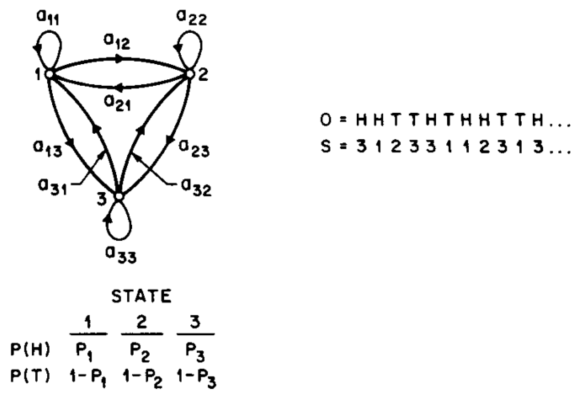
\includegraphics[width=0.56\textwidth]{hmm_coins}
        \caption{Example of a 3-coin model \cite{Rabiner1989}}
        \label{fig:hmm_coins}
    \end{center}
\end{figure}

A HMM is characterized by the following:
\begin{itemize}
    \item $ N $ which is the number of states in the model where individual 
    states are represented by $ S = \{ S_{1}, ..., S_{N} \} $ and the state at 
    time $ t $ is $ q_{t} $;
    \item $ M $ which is the number of distinct observation symbols per state 
    (individual symbols are represented by $ V = \{V_{1}, ..., V_{M} \} $);
    \item $ A = \{ a_{i, j} \} $, the state transition probability 
    distribution where
    \begin{equation}
    a_{ij} = p(q_{t+1} = S_{j} \mid q_{t} = S_{i}), 1 \leq i, j \leq N
    \end{equation}
    \item $ B = \{ b_{j}(k) \} $, the observation symbol probability 
    distribution in state $ j $:
    \begin{equation}
    b_{j}(k) = p(v_{k}~at \mid q_{t} = S_{j}), 1 \leq j \leq N, 1 \leq k 
    \leq M
    \end{equation}
    \item Finally, $ \pi = \{ \pi_{i} \} $, the initial state distribution:
    \begin{equation}
    \pi_{i} = p(q_{1} = S_{i}), 1 \leq i \leq N
    \end{equation}
\end{itemize}

The formal model can be summarized as $ \lambda = (A, B, \pi) 
$~\cite{Rabiner1989}.

Multiple algorithms have been studied and applied to HMMs: for inference, the 
forward algorithm, forward-backward algorithm \cite{baum1967inequality} or the 
Viterbi algorithm \cite{forney2005viterbi, martin2000speech}. Regarding 
learning, the algorithm Baum-Welch \cite{Baum1966, baum1967inequality} can be 
used.

Regarding e-commerce and web user behaviour there is some research done. 
\cite{Xie2009}~explains how to use a hidden semi-Markov model to detect 
anomalies on user browsing behaviour. \cite{Anderson2002}~describes very 
briefly a relational hidden Markov model for the behaviour of web site users, 
in order to improve predictions and personalization of websites.

\subsection{Summary}

In this section we reviewed the literature for graphical models. They provide a 
tool of excellence to model real world phenomena, enabling decision making 
under uncertainty and noisy observations.

There are multiple categories of graphical models however we focused on 
Bayesian and Markov networks and hidden Markov models, due to their 
applicability in the work at hand (in chapter \ref{chap:method} we will define 
how PGMs can be applied).
